\documentclass[a4paper, 12pt]{article}
\usepackage[margin=2cm,lmargin=4cm]{geometry}
\usepackage{parskip, indentfirst}

% Added for standalone images
\usepackage[subpreambles=true]{standalone}
% Added for code insertion
\usepackage{listings}

% added For Chinese Availablity
\usepackage{luatexja-fontspec}
\setmainjfont{FandolSong}

%Arial Narrow Font for front most page
\usepackage{fontspec}
\newfontfamily\arialnarrow[
    Path = ./fonts/,
    UprightFont = ARIALN.TTF,
    BoldFont = ARIALNB.TTF,
    ItalicFont = ARIALNI.TTF,
    BoldItalicFont = ARIALNBI.TTF
]{Arial Narrow}

\def\defparskip{0.5cm}
\def\defparindent{0.5cm}
\parskip=\defparskip
\parindent=\defparskip

\usepackage{newtxtext, newtxmath}

\usepackage{hyperref}
\usepackage{titlesec, titletoc, chngcntr}
\titleformat{\section}[hang]{\center\bfseries\MakeUppercase}{CHAPTER \thesection: }{0pt}{}
\titleformat*{\subsection}{\bfseries}
\titleformat*{\subsubsection}{\bfseries}

\titlecontents{figure}[0pt]{}{Figure \thecontentslabel: }{}{\titlerule*[9pt]{.}\contentspage}
\titlecontents{table}[0pt]{}{Table \thecontentslabel: }{}{\titlerule*[9pt]{.}\contentspage}
\counterwithin{figure}{section}
\counterwithin{table}{section}

\usepackage{graphicx, setspace, multicol, multirow, tikz, fancyhdr}
\usepackage{caption, subcaption, float, enumitem, blindtext}
\usepackage{amsmath, physics, siunitx}
\usepackage[]{apacite}

\fancyhead{}
\fancyfoot{}
\fancyfoot[R]{\fontsize{10pt}{10pt}\selectfont\thepage\normalsize}
\renewcommand{\headrulewidth}{0pt}

\setlist{parsep=0pt}
\sisetup{separate-uncertainty=true}
% The following line maxes out the figure size at \linewidth,
% you can always change the size you want by changing them per image
\setkeys{Gin}{width=\linewidth,keepaspectratio}
\captionsetup{width=0.8\linewidth, font=bf}
\numberwithin{equation}{section}
\usetikzlibrary{shapes,arrows.meta,positioning,calc}

% This part is added to allow subfigures
\captionsetup[subfigure]{labelformat=simple,justification=centerlast}

\renewcommand\thesubfigure{(\alph{subfigure})}
\makeatletter
\renewcommand\p@subfigure{\thefigure~}
\makeatother

% distance between floats
\setlength{\textfloatsep}{1cm plus 1.0pt minus 1.0pt}
\setlength{\intextsep}{1cm plus 1.0pt minus 1.0pt}
\setlength{\floatsep}{1cm plus 1.0pt minus 1.0pt}

\gdef\date{\today}
\gdef\title{YOUR THESIS TITLE}
\gdef\titleMS{YOUR THESIS TITLE IN MALAY}
\gdef\author{XXXXXXXX XXXXXX}
\gdef\matricno{XXXXXXXXX}
\gdef\IC{XXXXXX-XX-XXXX}
\gdef\degreename{Degree Xx Xxxxx Xxxxxxxxxxx}
\gdef\faculty{Xxxxxxxxxxx}

\begin{document}
\startcontents[default]

\pagestyle{empty}
\titlecontents{section}[0pt]{}{}{}{\titlerule*[9pt]{.}\contentspage}
\newgeometry{hmargin=4cm, vmargin=5cm}

\arialnarrow\bfseries
\fontsize{16pt}{16pt}\selectfont
\begin{center}
	\title
	\vfill
	\author
	\vfill
	FACULTY OF \MakeUppercase{\faculty}\\
	UNIVERSITI MALAYA\\
	KUALA LUMPUR

	\the\year
\end{center}

\clearpage

\rmfamily
\fontsize{14pt}{14pt}\selectfont
\begin{center}
	\title
	\vfill
	\author
	\vfill

	THESIS SUBMITTED IN FULFILMENT OF THE REQUIREMENTS
	FOR THE \MakeUppercase{\degreename}
	\vspace{2cm}

	FACULTY OF \MakeUppercase{\faculty}\\
	UNIVERSITI MALAYA\\
	KUALA LUMPUR

	\the\year
\end{center}

\normalfont
\clearpage
\normalsize
\restoregeometry

\pagestyle{fancy}
\pagenumbering{roman}
\setcounter{page}{2}
\parindent=0pt
\parskip=6pt

\begin{center}
	{\bfseries
		UNIVERSITI MALAYA

		ORIGINAL LITERARY WORK DECLARATION
	}
	\vspace{1cm}

\end{center}

Name of Candidate: \author\hfill (I.C/Passport No:\IC)

Matric No: \matricno

Name of Degree: \degreename

Title of Project Paper (``this Work''):

\title

Field of Study: Xxxxxxxxxxx
\vspace{1em}

I do solemnly and sincerely declare that:
\begin{enumerate}[label=(\arabic*)]
	\item I am the sole author of this Work;
	\item This Work is original;
	\item Any use of any work in which copyright exists was done by way of fair
	      dealing and for permitted purposes and any excerpt or extract from, or
	      reference to or reproduction of any copyright work has been disclosed expressly
	      and sufficiently and the title of the Work and its authorship have been
	      acknowledged in this Work;

	\item I do not have any actual knowledge nor do I ought reasonably to know that
	      the making of this work constitutes an infringement of any copyright work;

	\item I hereby assign all and every rights in the copyright to this Work to the
	      University of Malaya (``UM''), who henceforth shall be owner of the copyright in
	      this Work and that any reproduction or use in any form or by any means
	      whatsoever is prohibited without the written consent of UM having been first
	      had and obtained;

	\item I am fully aware that if in the course of making this Work I have infringed
	      any copyright whether intentionally or otherwise, I may be subject to legal
	      action or any other action as may be determined by UM.
\end{enumerate}
\vfill

\hspace{1cm}Candidate's Signature\hfill Date:\ \date
\vspace{.1in}

Subscribed and solemnly declared before,
\vfill

\hspace{1cm}Witness's Signature\hfill Date:\ \date

Name:

Designation:

\clearpage
\parskip=\defparskip
\parindent=\defparskip

\doublespacing
\phantomsection
\addcontentsline{toc}{section}{Abstract}

\begin{center}
	\bfseries
	\begin{singlespace}
		\title
	\end{singlespace}

	ABSTRACT
\end{center}

\blindtext[0]

\clearpage
\phantomsection
\addcontentsline{toc}{section}{Abstrak}

\begin{center}
	\bfseries
	\begin{singlespace}
		\titleMS
	\end{singlespace}

	ABSTRAK
\end{center}

\blindtext[0]

\clearpage
\onehalfspacing

\phantomsection
\addcontentsline{toc}{section}{Acknowledgements}

\begin{center}
	\bfseries
	ACKNOWLEDGEMENTS
\end{center}

\blindtext[0]
\clearpage


\parskip=0pt
\parindent=0pt
\doublespacing

\renewcommand{\contentsname}{Table of Contents}
\phantomsection
\section*{\contentsname}
\addcontentsline{toc}{section}{\contentsname}
% This allows printing up to \subsubsectionin content 
\printcontents[default]{l}{0}{\setcounter{tocdepth}{3}}
\clearpage

\phantomsection
\addcontentsline{toc}{section}{\listfigurename}
\listoffigures
\clearpage

\phantomsection
\addcontentsline{toc}{section}{\listtablename}
\listoftables
\clearpage

\phantomsection
\xdef\listsymbolname{List of Symbols and Abbreviations}
\section*{\listsymbolname}
\addcontentsline{toc}{section}{\listsymbolname}
\begin{tabular}{l>{:\hspace{0.5cm}}l}
	EA & Example Abbreviation
\end{tabular}
\clearpage

\phantomsection
\xdef\listappendixname{List of Appendices}
\section*{\listappendixname}
\addcontentsline{toc}{section}{\listappendixname}
\startcontents[appendix]
\printcontents[appendix]{l}{0}{\setcounter{tocdepth}{2}}
\stopcontents[appendix]
\clearpage

\parskip=1cm
\parindent=0.5cm

\doublespacing
\parindent=0.5cm
\parskip=0.5cm
\pagenumbering{arabic}
\titlecontents{section}[0pt]{\vspace*{1cm}}{\bfseries CHAPTER \thecontentslabel: \uppercase}{}{\titlerule*[9pt]{ }\contentspage}

\section{Introduction}

This is introduction \shortcite{example2002}.

\subsection{Problem Statement}

Example.

\subsection{Research Questions}

The research aims to answer the following questions:
\begin{enumerate}
	\item Example.
\end{enumerate}

\subsection{Research Objectives}

The research aims to achieve the following objectives:
\begin{enumerate}
	\item Example.
\end{enumerate}

\subsection{Relevance of Research}

Example.

\clearpage
\section{Literature Review}
\subsection{Subtopics}

Your literature review content goes here. This section should contain your analysis and discussion of relevant academic sources.

% ==========================================
% FIGURE EXAMPLES
% ==========================================

% Single Figure Example
\begin{figure}[H]
    \centering
    % Adjust image width using the width parameter (default is full linewidth)
    
\includegraphics[width=0.2\linewidth]{assets/example.png}
    \caption{Example figure with citation\protect\shortcite{example2002}}
    \label{fig:example}
\end{figure}

% Reference the figure in text
As shown in Figure~\ref{fig:example}, ...

% ==========================================
% SUBFIGURE EXAMPLES
% ==========================================

% Multiple Subfigures with Independent Sizing
\begin{figure}[H]
    \centering
    % Subfigure A
    \subcaptionbox{Sub Figure A\label{fig:subfigure_a}}{
        
\includegraphics[width=0.2\linewidth]{assets/example.png}
    }
    % Subfigure B
    \subcaptionbox{Sub Figure B\label{fig:subfigure_b}}{
        
\includegraphics[width=0.4\linewidth]{assets/example.png}
    }
    % Subfigure C
    \subcaptionbox{Sub Figure C\label{fig:subfigure_c}}{
        
\includegraphics[width=0.3\linewidth]{assets/example.png}
    }
    \caption{Comprehensive figure showing multiple related elements.}
    \label{fig:whole_figure}
\end{figure}

% Reference subfigures in text
Figure~\ref{fig:whole_figure} presents a comprehensive view consisting of 
Figure~\ref{fig:subfigure_a}, Figure~\ref{fig:subfigure_b}, and Figure~\ref{fig:subfigure_c}.

% ==========================================
% TABLE EXAMPLES
% ==========================================

\begin{table}[H]
    \centering
    \caption{Example table with clear headers and data.}
    \label{tab:example}
    \begin{tabular}{|c|c|}
        \hline
        \textbf{Column A} & \textbf{Column B} \\
        \hline
        Data 1 & Data 2 \\
        \hline
        Data 3 & Data 4 \\
        \hline
    \end{tabular}
\end{table}

% Reference the table in text
The results presented in Table~\ref{tab:example} demonstrate...

% ==========================================
% TIKZ STANDALONE EXAMPLES
% ==========================================

% TikZ Flowchart/Diagram Example
\begin{figure}[H]
    \centering
    % Resize to fit within specified height while maintaining aspect ratio
    \resizebox{!}{0.3\textheight}{
        \documentclass[tikz,border=10pt]{standalone}
\usepackage{tikz}
\usetikzlibrary{positioning,arrows.meta,shapes.geometric,shapes.misc,calc}
\begin{document}
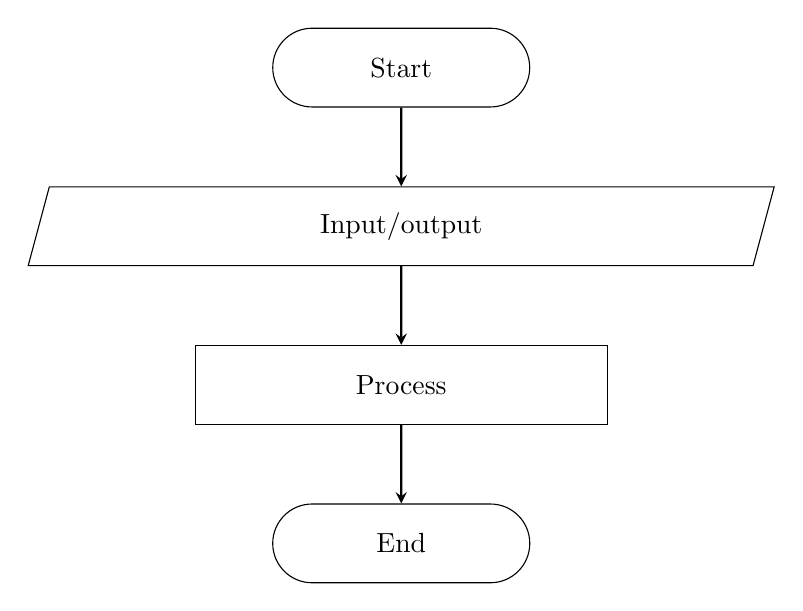
\begin{tikzpicture}[
    node distance=1cm,
    start_end/.style={  
        rounded rectangle,% Rounded rectangle shape  
        draw,  
        text centered,  
        minimum height=1cm,  
        text width=3cm,  
    },  
    process/.style={rectangle, draw, text width=5cm, text centered, minimum height=1cm},
    io/.style={trapezium, trapezium left angle=75, trapezium right angle=105, draw, text width=5cm, minimum width=4.8cm, trapezium stretches=false, text centered, minimum height=1cm},
    arrow/.style={thick, ->, >=stealth}
]
    
    % Nodes
    \node[start_end] (start) {Start};
    \node[io, below=of start] (io) {Input/output};
    \node[process, below=of io] (process) {Process};
    
    \node[start_end, below=of process] (end) {End};
    
    % Connections   
    \draw[arrow] (start) -- (io);
    \draw[arrow] (io) -- (process);
    \draw[arrow] (process) -- (end);
\end{tikzpicture}
\end{document}
    }
    \caption{Example flowchart demonstrating the methodology.}
    \label{fig:example_flowchart}
\end{figure}

% Reference the flowchart in text
The methodology outlined in Figure~\ref{fig:example_flowchart} illustrates...

% ==========================================
% APPENDIX REFERENCES
% ==========================================

% Reference to appendix material
Additional detailed information can be found in Appendix~\ref{app:example}.
\clearpage
\section{Methodology}


\clearpage
\section{Results}

\clearpage
\section{Discussion}

\clearpage
\section{Conclusion}

\clearpage

\titlecontents{section}[0pt]{\vspace*{1cm}}{}{}{\titlerule*[9pt]{.}\contentspage}

\singlespacing
\setlength{\bibitemsep}{\baselineskip}
\phantomsection
\bibliographystyle{apacite}
\bibliography{ref.bib}
\clearpage

\stopcontents[default]
\resumecontents[appendix]
\appendix
\titleformat{\section}[hang]{\center\bfseries\MakeUppercase}{APPENDIX \thesection: }{0pt}{}
\titlecontents{section}[0pt]{}{Appendix \thecontentslabel: }{}{\titlerule*[9pt]{.}\contentspage}

% Remove or comment the next line if you don't have any appendix
\section{Example Appendix}
\label{app:example}
You can put your data here if needed

\stopcontents[appendix]
\end{document}
